\documentclass[11pt,a4paper]{article}
\usepackage[T1]{fontenc}
\usepackage[utf8]{inputenc}
\usepackage{lmodern}
\usepackage[margin=25mm]{geometry}
\usepackage{amsmath,amssymb,booktabs,array,longtable,tabularx}
\usepackage{graphicx,xcolor,microtype,xurl}
\usepackage[numbers,sort&compress]{natbib}
\usepackage[colorlinks=true,linkcolor=blue!45!black,citecolor=blue!45!black,urlcolor=blue!45!black]{hyperref}
\hypersetup{pdftitle={GatedV: Self-Gated Values for Transformer Language Models},pdfauthor={Li-Ming Yu },pdfsubject={GatedV},pdfkeywords={Transformer, value projection, SiLU, paired experiments}}
\usepackage{enumitem,placeins}
\setlist{nosep,leftmargin=*}
\setlength{\parskip}{3pt}
\setlength{\parindent}{1em}
\setlength{\emergencystretch}{2em}
\newcommand{\silu}{\operatorname{SiLU}}
\newcommand{\rms}{\operatorname{RMSNorm}}
\newcommand{\softmax}{\operatorname{softmax}}
\newcommand{\E}{\mathbb{E}}
\newcommand{\vonly}{GatedV}
\newcommand{\code}[1]{\texttt{\small #1}}
\newcommand{\minus}{\ensuremath{-}}
\title{GatedV: Self-Gated Values for Transformer Language Models}
\author{
  Li-Ming Yu\thanks{Email:
    \href{mailto:yuliming1996@gmail.com}
    {\texttt{yuliming1996@gmail.com}}; ORCID:
    \href{https://orcid.org/0000-0001-7552-8895}
    {0000-0001-7552-8895}.}\\
  Independent Researcher
}

\begin{document}
\maketitle
\begin{abstract}

Standard attention forms query (Q), key (K), and value (V) matrices through learned linear projections of input hidden states. Architectures such as GAU and Mega incorporate nonlinear transformations into attention. In this paper, we propose \textbf{GatedV}, a simple attention variant that applies SiLU only to V before aggregation without introducing additional trainable parameters. We evaluate GatedV against a standard decoder-only Transformer using matched parameter counts, paired initializations, and equal training-token budgets. At 2.33M parameters, GatedV reduces mean held-out perplexity from 59.1 to 57.9 (2.0\%), with improvements across all five paired seeds. At 26.16M parameters, following an equal-budget learning-rate search, mean held-out perplexity falls from 21.4 to 20.6 (3.7\%), with improvements across all three paired seeds. Small-model ablations show that the tested affine rescaling of values does not fully reproduce GatedV's gains. A short interleaved benchmark on NVIDIA DGX Spark measures approximately 0.7\% higher full-context forward latency for the larger model, based on synchronized wall-clock timings. These findings suggest that value-only self-gating can improve language modeling performance without increasing parameter count or redesigning the attention-weighting mechanism.
\end{abstract}

\section{Introduction}

Standard Transformer blocks combine self-attention with position-wise feed-forward networks~\citep{transformer}. The feed-forward sublayer applies nonlinear transformations to individual token representations, whereas attention mixes information across tokens. Within attention, queries (Q) and keys (K) determine the mixing weights, and values (V) provide the representations to be combined. These three branches are usually formed by linear projections, despite their different roles. An additional nonlinearity on queries or keys changes the weighting calculation; on values, it changes what enters the weighted sum. Moreover, applying a nonlinearity before aggregation is generally not equivalent to applying it afterward.

Nonlinear value representations are already used in several attention architectures. Mega applies SiLU to projected values in a block that also uses moving-average features and additional gates~\citep{mega}. HYLA introduces nonlinear value computation without additional parameters, together with normalization across attention heads~\citep{hypernetwork}. Neural Attention instead replaces the linear Q/K/V projections with multilayer perceptrons~\citep{neuralattention}. Gated Attention compares gates at several locations, including the value projection, with its main results using a learned sigmoid gate after scaled dot-product attention~\citep{gatedattention}. GLU Attention introduces separate content and gate projections and reduces the aggregated value width to match the combined value/output projection-weight count~\citep{gluattention}. These approaches differ in both the source of the nonlinearity and the computation surrounding it.

A narrower question is whether a nonlinear value transform improves a standard Transformer when the other components are left unchanged. Matching parameter counts by narrowing projections also changes the dimensions of the value representation. A parameter-free elementwise activation allows the original projection dimensions and block configuration to be retained, while altering only the operation applied to the projected values.

We call this variant \textbf{GatedV} (self-gated values). It applies SiLU to the usual value projection $V$ before attention aggregation:
\[
    \widetilde V=\silu(V)=V\odot\sigma(V),
\]
where $\sigma$ is the elementwise sigmoid function. The same projected values supply both the content and its gate, so no separate learned gate projection is needed. The query/key projections, softmax weighting rule, and remaining Transformer components are retained. GatedV therefore has exactly the same number of trainable parameters as the baseline, without adjusting the depth or width of either model.

We train baseline and GatedV decoder-only language models from scratch on FineWeb-Edu~\citep{fineweb}, at 2.33M and 26.16M parameters and with equal training-token budgets within each scale. GatedV reduces mean held-out perplexity by 2.0\% and 3.7\%, respectively, with improvements in every paired confirmation run. Additional experiments examine activation placement, learning-rate sensitivity, initial value statistics, and computational cost. Whether these improvements persist at larger scales, on other corpora, or on tasks beyond next-token prediction remains to be tested.

Code, experiment recipes, and recorded results are available at \url{https://github.com/yuliming1996/GatedV}.


\section{Background and model formulation}
\label{sec:background}

\subsection{Transformer backbone}
\label{sec:backbone}
Our baseline is a decoder-only Transformer with causal multihead attention~\citep{transformer,gpt}. Each block uses RMSNorm before its attention and feed-forward sublayers~\citep{rmsnorm}, rotary positional embeddings for queries and keys~\citep{rope}, and a SwiGLU feed-forward transformation~\citep{swiglu}.

Let $X\in\mathbb{R}^{T\times d}$ denote the hidden states entering a block, where $T$ is the sequence length and $d$ is the model width. We omit the batch dimension and use row-vector notation. The attention sublayer first computes
\begin{equation}
 U=\rms_{\gamma_a}(X),\qquad
 Q=UW_Q,\quad K=UW_K,\quad V=UW_V,
 \label{eq:projections}
\end{equation}
where $W_Q,W_K,W_V\in\mathbb{R}^{d\times d}$. RMSNorm acts on each token independently:
\begin{equation}
 \rms_\gamma(x)=\gamma\odot
 \frac{x}{\sqrt{d^{-1}\sum_{j=1}^{d}x_j^2+\epsilon}},
 \qquad \epsilon=10^{-6}.
 \label{eq:rmsnorm}
\end{equation}
The projected tensors are split into $H$ heads of width $d_h=d/H$. For head $h$, let $\widehat Q_h=\operatorname{RoPE}(Q_h)$ and $\widehat K_h=\operatorname{RoPE}(K_h)$. We use a rotary base of 10,000. The attention weights and output are
\begin{equation}
 A_h=\softmax\!\left(
 \frac{\widehat Q_h\widehat K_h^\top}{\sqrt{d_h}}+M
 \right),\qquad
 O=\operatorname{Concat}_{h=1}^{H}(A_hV_h),
 \label{eq:attention}
\end{equation}
where $M_{ij}=0$ for $j\leq i$ and $M_{ij}=-\infty$ otherwise. Softmax is applied across the key positions in each row. Values enter this aggregation linearly for fixed $A_h$, although attention as a function of $X$ is nonlinear because the weights themselves depend on the input.

The block then applies the two residual updates
\begin{align}
 X'&=X+OW_O,\\
 Z&=\rms_{\gamma_f}(X'),\\
 X_{\mathrm{next}}&=X'+
 \big[\silu(ZW_1)\odot(ZW_2)\big]W_3,
 \label{eq:block}
\end{align}
where $W_O\in\mathbb{R}^{d\times d}$, $W_1,W_2\in\mathbb{R}^{d\times d_{\mathrm{ff}}}$, and $W_3\in\mathbb{R}^{d_{\mathrm{ff}}\times d}$. The SiLU activation is $\silu(z)=z\sigma(z)$, with $\sigma(z)=(1+e^{-z})^{-1}$~\citep{silu,swish}; both the activation and $\odot$ act elementwise. After $L$ blocks, a final RMSNorm precedes the vocabulary readout, whose weights are tied to the input embedding. All learned linear maps are bias-free. Dropout and additional headwise query/key normalization are disabled.

\subsection{Nonlinear projections and attention gates}
\label{sec:related}
Nonlinear features can be introduced at several stages of attention, beginning with the projections that construct Q, K, and V. Neural Attention replaces these linear maps with two-layer networks containing LayerNorm and ReLU~\citep{neuralattention}. This increases the projection parameter count. Its ReLU ablation retains the expanded key/value projections and LayerNorm, testing the activation within the modified network rather than comparing with a parameter-matched standard Transformer.

Nonlinear values also appear in architectures that redesign the attention block more broadly. The Gated Attention Unit (GAU) combines nonlinear values and shared query/key features with squared-ReLU attention and multiplicative gating in a unified attention and feed-forward layer~\citep{gau}. Mega builds on this construction, deriving shared query/key features from exponential moving averages and adding reset and update gates~\citep{mega}. Its value branch applies SiLU directly to the projected inputs before aggregation. This provides a direct precedent for value-side SiLU, although the surrounding computation differs from conventional multihead attention.

GLU Attention retains softmax aggregation and uses two independently projected branches, $\widetilde V=(UW_C)\odot\silu(UW_G)$~\citep{gluattention}. For model width $d$, it sets the combined value width across heads to $m=2d/3$. Ignoring biases, the two $d\times m$ input projections and the $m\times d$ output projection then contain $3dm=2d^2$ weights, matching the standard value and output projections. Thus its parameter matching involves narrower values and a separate learned gate. GatedV instead preserves the original value width and projection matrices, applying SiLU directly to a single projected value tensor.

Other formulations make the nonlinear transformation depend on how values are combined. HYLA applies ReLU to an attention-weighted combination of value features across heads for each query--key pair. It introduces no additional parameters and uses RMS normalization across heads instead of key-wise softmax~\citep{hypernetwork}. LASER retains softmax weights but combines an exponential value transform with a logarithm after aggregation, giving $\log\!\big(A_h\exp(V_h)\big)$~\citep{laser}. These operations are not generally equivalent to applying an activation independently to each projected value and then taking the usual weighted sum.

Gate placement has also been studied while retaining softmax attention. Gated Attention compares learned gates on Q/K/V and at the attention output, with its main configuration using a head-specific sigmoid gate after scaled dot-product attention~\citep{gatedattention}. It also evaluates SiLU applied directly to the attention output without additional parameters. Two distinctions are relevant here: whether the gate uses a separate learned projection, and whether it acts before or after aggregation. We examine self-gating of the projected values before aggregation, retaining the original projections and the softmax weighting rule.

\subsection{GatedV}
\label{sec:model}
GatedV replaces the projected values in Equation~\ref{eq:projections} with
\begin{equation}
 \widetilde V=\phi(V)=V\odot\sigma(V),
 \qquad \phi=\silu.
 \label{eq:selfgate}
\end{equation}

\begin{figure}[t]
\centering
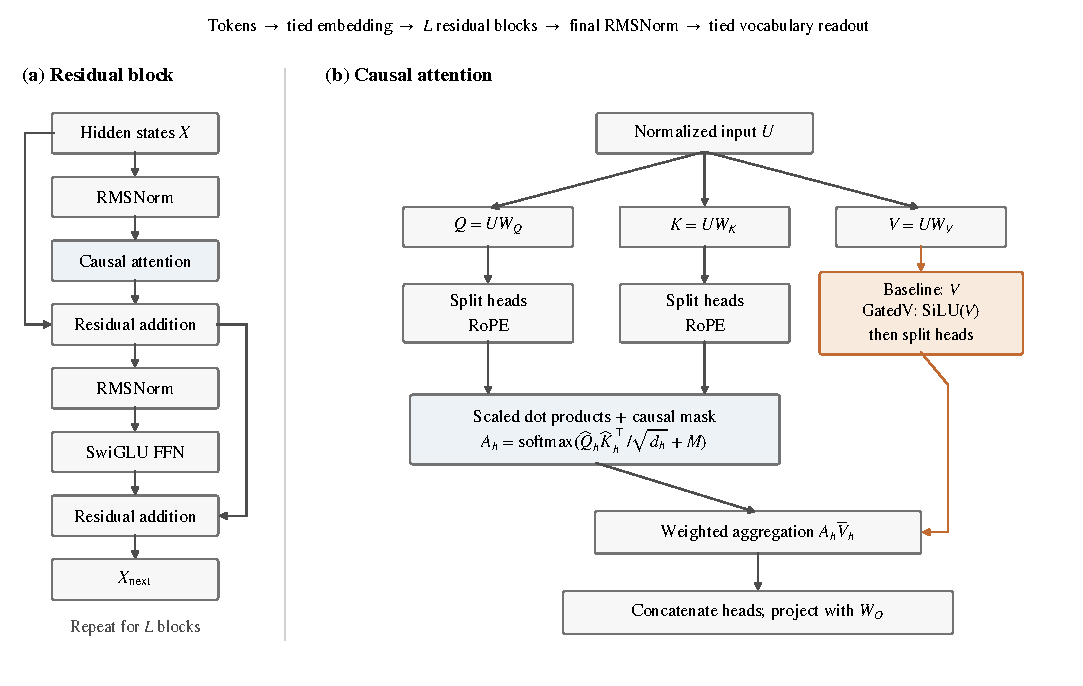
\includegraphics[width=\linewidth]{figures/architecture_gatedv.pdf}
\caption{Transformer block and GatedV value transformation. The baseline aggregates the projected values $V$, whereas GatedV applies $\silu(V)$ before aggregation. Queries and keys receive RoPE before score construction. The value box shows the two model variants; only one is used in each model. The Q/K/V projections are drawn separately but implemented as one fused bias-free linear map.}
\label{fig:architecture}
\end{figure}

The Q/K/V projections are implemented as one fused linear map. After splitting its output into three tensors, we apply $\phi$ to $V$ before reshaping into heads. The per-head comparison is therefore
\begin{equation}
 Y_h^{\mathrm{base}}=A_hV_h,\qquad
 Y_h^{\text{GatedV}}=A_h\phi(V_h).
 \label{eq:vonly}
\end{equation}
Figure~\ref{fig:architecture} shows where the value activation is applied.

The gate is determined by the same projected value that it multiplies. It requires no separate projection such as $W_G$ in $(UW_V)\odot\sigma(UW_G)$, the two-projection form of a gated linear unit~\citep{glu}. Its placement also matters: in general,
\begin{equation}
 A_h\phi(V_h)\neq\phi(A_hV_h).
 \label{eq:placement}
\end{equation}
The left-hand side transforms each source token's value before mixing it with other values; the right-hand side transforms the resulting mixture.

For a fixed normalized input $U$ and fixed query/key projection weights, GatedV leaves $A_h$ unchanged. This is a local property of the computation, not a claim that trained models have identical attention patterns. The altered values change the inputs to later layers, and the activation also changes the gradients through the value projection.

No trainable tensors are added or resized. The depth, hidden widths, head structure, normalization, positional encoding, and feed-forward blocks remain as defined above, so paired baseline and GatedV models can start from identical weights. The activation adds $O(Td)$ elementwise work per block; the $O(T^2d)$ cost of full attention is unchanged. Equal parameter counts thus do not imply equal computational cost.

For the activation-placement experiments, we also apply $\phi$ to queries alone or to all three of Q, K, and V. Query and key activations are applied before RoPE. These variants retain the original depth and projection dimensions.

\FloatBarrier

\section{Experimental design}
\label{sec:experiments}

\subsection{Models, data, and training}
\label{sec:training}
We compare the baseline and GatedV at two model sizes (Table~\ref{tab:backbone}). Within each comparison, the models have the same architecture apart from the value activation, start from identical trainable weights, and process the same sampled windows in the same order. Paired seeds and separate learning-rate selection address sources of benchmark variation~\citep{benchvariance}.

\begin{table}[t]
\centering\small
\caption{Main confirmation settings. Both models use a vocabulary of 8,192, context length 256, and batch size 8. Target exposures count sampled prediction targets, including repetitions.}
\label{tab:backbone}
\begin{tabular}{lrr}
\toprule
Setting & Small & Medium\\
\midrule
Layers / model width & 6 / 128 & 12 / 384\\
Heads / head width & 4 / 32 & 6 / 64\\
SwiGLU hidden width & 384 & 1,152\\
Trainable parameters & 2,328,192 & 26,158,464\\
Training-corpus tokens & 40,001,310 & 512,000,068\\
Training-corpus documents & 27,830 & 212,052\\
Updates per run & 32,768 & 327,680\\
Target exposures per run & 67,108,864 & 671,088,640\\
Warmup updates & 512 & 5,120\\
Confirmation peak learning rate & 0.0048 & 0.0006\\
Paired confirmation seeds & 5 & 3\\
\bottomrule
\end{tabular}
\end{table}

All model training uses FineWeb-Edu text~\citep{fineweb}. The tokenizer is a fixed 8,192-entry byte-level BPE tokenizer~\citep{gpt2}, previously trained on a WikiText training split~\citep{wikitext}; it is not fitted to the evaluation sets. The medium corpus was prepared before this study and reused. Each training window remains within one document and supplies 256 next-token targets. An update therefore contains 2,048 target exposures, but may revisit previously sampled text.

The small confirmation uses 2,048 held-out documents, one per domain group, with 524,288 targets in total. The medium study uses separate development and held-out sets of the same size. Each document contributes its first eligible 256-target window. Evaluation preparation excludes the current training corpus and registered historical datasets through identity, URL, domain, exact-text, normalized-text, near-duplicate, and long-fragment checks. Such overlap checks address known risks in language-model evaluation~\citep{dedup}, but cannot guarantee the absence of all semantic overlap. The small-model exploratory studies and confirmation learning curves use a reused development cohort of 352 documents in 254 domain groups, with 131,072 evaluated targets.

Training uses AdamW~\citep{adamw} with $(\beta_1,\beta_2)=(0.9,0.95)$, $\epsilon=10^{-8}$, weight decay 0.1 on all matrix parameters, and no decay on normalization gains. The global gradient norm is clipped to 1. Learning rates warm up and then follow a cosine schedule to 10\% of the peak. All reported endpoints are the final fixed-budget checkpoints, not the best intermediate checkpoints. The main comparisons run in FP32 on DGX Spark with deterministic mathematical scaled-dot-product attention; autocast, TF32, and compilation are disabled. Gaussian initialization uses fan-in scaling and seeds derived from parameter names, with separate seeds for the fused Q/K/V chunks. Output and feed-forward down-projections are scaled by $1/\sqrt{2L}$, and normalization gains start at one.

\subsection{Confirmations and exploratory comparisons}
The research sequence was adaptive, but each confirmation used new paired seeds and a held-out set excluded from model and learning-rate selection. The small confirmation fixed GatedV and a shared peak learning rate of 0.0048 after an activation-placement screen with 4,096 updates per run and rates $\{0.0012,0.0024,0.0048\}$. The screen compared the baseline with query-only, value-only, and joint Q/K/V SiLU, followed by three-seed rechecks at 32,768 updates. The small confirmation evaluates the two architectures at the fixed learning rate; it does not optimize the rate separately for each model.

For the medium model, each architecture receives one full-budget run at each rate in $\{0.0006,0.0012,0.0024\}$, using the same selection seed. The lowest final development NLL selects the rate for each architecture, with ties resolved toward the lower rate. Neither the learning-rate grid nor the training budget is extended. After selection, three new paired seeds are trained from scratch at the selected rates. Held-out evaluation follows completion of all six confirmation runs.

Three exploratory comparisons help interpret the results. First, we compare SiLU on queries alone, values alone, and all three projections at the same six-layer depth. Second, a three-seed, long-budget learning-rate study compares baseline and GatedV at $\{0.0012,0.0024,0.0048,0.0096\}$. The lowest rate was added after the original grid selected its lower boundary; these results reuse development data and are not an independent confirmation. Third, two fixed, parameter-free controls test initial value statistics: an affine transform matches the baseline values to the initial SiLU mean and variance, while a rescaled SiLU matches the original baseline moments. Each control receives two rates, 0.0024 and 0.0048. For each seed and layer, calibration uses 128 training windows processed by an initialized baseline without updates, pooling moments over windows, positions, and channels in FP64. Writing $(\mu_V,\sigma_V)$ and $(\mu_\phi,\sigma_\phi)$ for the moments of $V$ and $\phi(V)$, the two controls are
\begin{align}
 V_{\mathrm{aff}}&=\frac{\sigma_\phi}{\sigma_V}(V-\mu_V)+\mu_\phi,\\
 V_{\mathrm{mm}}&=\frac{\sigma_V}{\sigma_\phi}\big(\phi(V)-\mu_\phi\big)+\mu_V.
 \label{eq:controls}
\end{align}
The coefficients are frozen FP32 buffers; moment matching is local to the calibration inputs and is not maintained during training.

\subsection{Evaluation and uncertainty}
For seed $s$, document loss sums $\ell_{s,i}$, and target counts $n_i$, we report token-averaged negative log-likelihood and perplexity as
\begin{equation}
 L_s=\frac{\sum_i\ell_{s,i}}{\sum_i n_i},\qquad P_s=\exp(L_s),\qquad
 \Delta_P=100\left(\frac{\overline P_{\mathrm{GatedV}}}{\overline P_{\mathrm{base}}}-1\right).
 \label{eq:pplchange}
\end{equation}
Logarithms are natural, and $\overline P$ is the arithmetic mean of per-seed perplexities, not the exponential of mean NLL. Negative $\Delta_P$ denotes improvement. Unless stated otherwise, $\pm$ denotes sample standard deviation across training seeds.

We distinguish retraining variability from uncertainty over evaluation documents~\citep{benchvariance,statsguide}. For $S$ paired NLL differences $d_s=L_{\mathrm{GatedV},s}-L_{\mathrm{base},s}$, approximate 95\% intervals are $\overline d\pm t_{0.975,S-1}\operatorname{SD}(d)/\sqrt S$. The normality assumption is uncertain at these sample sizes. Domain-bootstrap intervals instead condition on the trained models. We average document loss differences across trained pairs, resample domain groups with replacement 2,000 times, and recompute the token-weighted mean difference. The 2.5th and 97.5th percentiles define the interval. In the main held-out sets, each domain contains one document, so domain and document resampling are the same partition, not independent evidence. Bootstrap intervals for mean NLL differences are not intervals for the arithmetic mean-PPL ratio. The small seed counts and adaptive exploration limit inference; no multiplicity-adjusted claim is made.

\section{Results}
\label{sec:results}

\subsection{Held-out language modeling}
Table~\ref{tab:confirmation} summarizes the two confirmations. At 2.33M parameters, mean held-out PPL decreases by 2.03\%, with all five pairs improving. Individual reductions range from 0.33\% to 3.74\%. At 26.16M parameters, both architectures select 0.0006, the lower boundary of the medium learning-rate grid. Three new confirmation pairs all improve, reducing mean held-out PPL by 3.66\%. The smaller observed GatedV seed variance at this scale is descriptive, not evidence of generally more stable training.

\begin{table}[t]
\centering\small
\caption{Held-out confirmation results. Values are arithmetic mean PPL $\pm$ sample SD. The studies use different held-out sets and training configurations.}
\label{tab:confirmation}
\begin{tabular}{lrrrr}
\toprule
Model size & Baseline & GatedV & $\Delta_P$ & Improved pairs\\
\midrule
2.33M & $59.118\pm0.530$ & $57.916\pm0.782$ & $-2.03\%$ & 5/5\\
26.16M & $21.384\pm0.166$ & $20.600\pm0.018$ & $-3.66\%$ & 3/3\\
\bottomrule
\end{tabular}
\end{table}

The mean paired NLL differences are $-0.020591$ and $-0.037317$ nats/token. Their approximate seed-level 95\% intervals are $[-0.036406,-0.004776]$ and $[-0.054554,-0.020079]$, respectively. Conditional domain-bootstrap intervals are narrower: $[-0.021869,-0.019356]$ and $[-0.038583,-0.036011]$. They quantify evaluation-set variation for these trained pairs and do not replace the seed intervals.

Figures~\ref{fig:development_delta_ppl} and~\ref{fig:development_ppl} show development perplexity during the confirmation runs. At each recorded update $u$, we exponentiate each run's development NLL and then average PPL across seeds. The paired difference is $\delta_s(u)=P_{\mathrm{GatedV},s}(u)-P_{\mathrm{base},s}(u)$, measured in PPL units; it is distinct from the percentage change $\Delta_P$ in Table~\ref{tab:confirmation}. Mean development PPL is lower for GatedV at all 16 post-initialization checkpoints at both scales, although individual small-model pairs do not improve at every checkpoint. Final development means are 58.716 versus 57.422 for the small model and 21.804 versus 21.039 for the medium model. These evaluations use development cohorts separate from the held-out sets in Table~\ref{tab:confirmation}.

\begin{figure}[t]
\centering
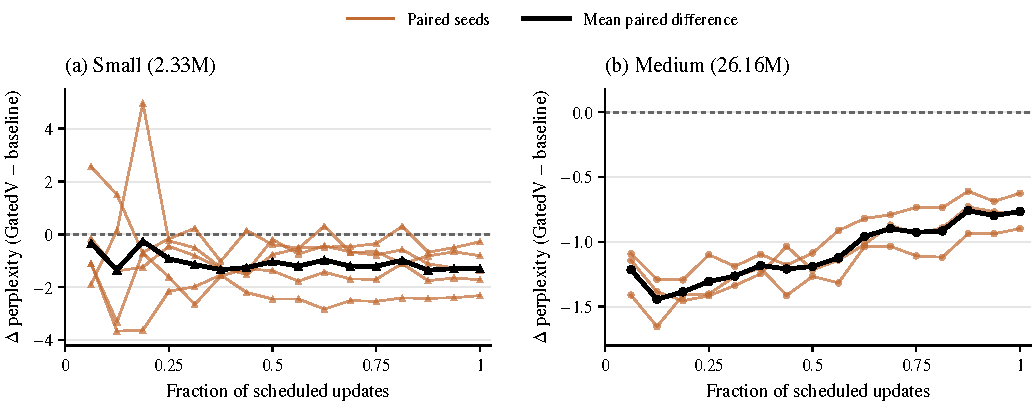
\includegraphics[width=\linewidth]{figures/development_delta_ppl.pdf}
\caption{Paired development PPL differences during training: GatedV minus baseline, with negative values favoring GatedV. Panels show the small and medium confirmations. Thin colored curves represent individual seed pairs; the thick black curve is their arithmetic mean. The horizontal axis is the fraction of each study's scheduled optimizer updates. All 16 post-initialization evaluations are shown, with no smoothing. Initialization is omitted from this view because its much larger differences obscure the training trajectories. These are development-set differences, not held-out scores.}
\label{fig:development_delta_ppl}
\end{figure}

\begin{figure}[t]
\centering
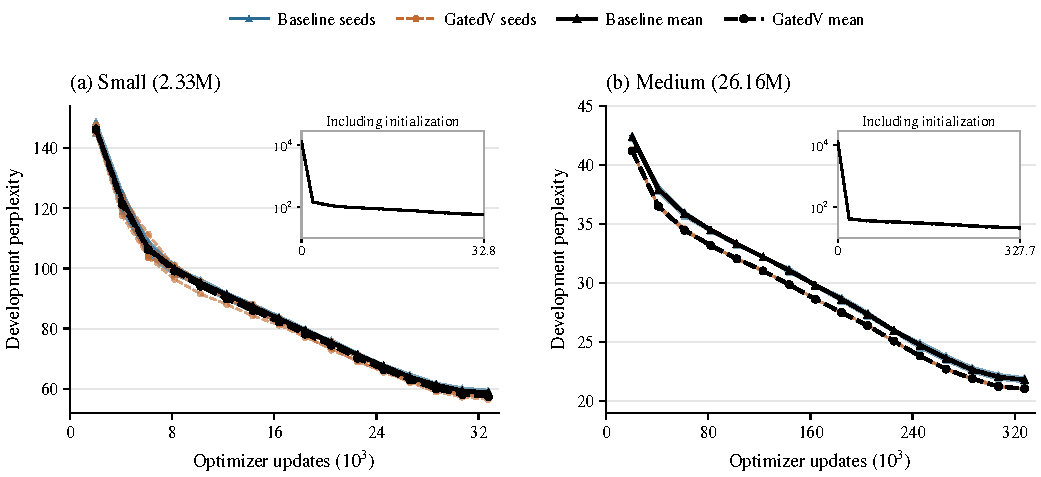
\includegraphics[width=\linewidth]{figures/development_ppl.pdf}
\caption{Development PPL versus optimizer updates for the small and medium confirmations. Thin blue and orange curves show individual baseline and GatedV runs, respectively. Thick black curves show arithmetic means across five small-model or three medium-model seeds; solid lines with filled triangles denote baseline, and dashed lines with filled circles denote GatedV. Main panels show all 16 post-initialization checkpoints on a linear scale. Insets include initialization and all subsequent checkpoints on a logarithmic PPL scale. Lines connect recorded evaluations without smoothing; held-out endpoints are reported separately in Table~\ref{tab:confirmation}.}
\label{fig:development_ppl}
\end{figure}

\subsection{Activation placement and learning rate}
Table~\ref{tab:ablations} separates the exploratory activation and learning-rate comparisons from medium-model selection. At the same six-layer depth, value-only SiLU improves all three pairs. Query-only SiLU worsens all three, while joint Q/K/V SiLU yields a small mean improvement in two pairs; its conditional bootstrap interval crosses zero. Thus the joint result is inconclusive, rather than evidence of equivalence to the baseline. Favorable short-screen rankings for query-only and joint activation do not persist at the longer budget. Because the learning-rate schedules depend on the training horizon, the short and long runs are separate training runs, not continuations of one trajectory.

\begin{table}[t]
\centering\small
\caption{Development-set comparisons. The first two groups use three seeds and 32,768 updates per run on reused development data; the last uses one selection seed and 327,680 updates on new development data. $\Delta_P$ compares the variant with the baseline in the same row.}
\label{tab:ablations}
\begin{tabular}{lrrrr}
\toprule
Variant or peak LR & Baseline PPL & Variant PPL & $\Delta_P$ & Improved pairs\\
\midrule
\multicolumn{5}{l}{\textit{Activation placement; shared LR 0.0048}}\\
Q-only & $58.580\pm0.557$ & $59.522\pm0.337$ & $+1.61\%$ & 0/3\\
GatedV & $58.580\pm0.557$ & $58.039\pm0.525$ & $-0.92\%$ & 3/3\\
All Q/K/V & $58.580\pm0.557$ & $58.458\pm0.485$ & $-0.21\%$ & 2/3\\
\midrule
\multicolumn{5}{l}{\textit{Small-model LR study; variant is GatedV}}\\
0.0012 & $56.441\pm0.548$ & $55.269\pm1.120$ & $-2.08\%$ & 2/3\\
0.0024 & $56.180\pm0.462$ & $54.450\pm0.140$ & $-3.08\%$ & 3/3\\
0.0048 & $58.770\pm0.983$ & $57.384\pm0.168$ & $-2.36\%$ & 3/3\\
0.0096 & $65.168\pm1.333$ & $64.063\pm0.442$ & $-1.70\%$ & 2/3\\
\midrule
\multicolumn{5}{l}{\textit{Medium-model LR selection; variant is GatedV}}\\
0.0006 & 21.558 & 21.005 & $-2.57\%$ & --\\
0.0012 & 23.707 & 23.161 & $-2.30\%$ & --\\
0.0024 & 27.691 & 30.213 & $+9.11\%$ & --\\
\bottomrule
\end{tabular}
\end{table}

In the long-budget small-model grid, both architectures select the interior rate 0.0024 by mean final development NLL. GatedV improves mean PPL by 3.08\% there and improves every pair. Its mean is favorable at all four rates, but one pair worsens at each of 0.0012 and 0.0096. Medium-model selection also shows learning-rate dependence: GatedV is worse at 0.0024. The gains are therefore not uniform across rates, and neither finite search establishes a global optimum.

Neither initialization-moment control reproduces the raw SiLU result (Table~\ref{tab:moment}). Both controls are worse than GatedV in every paired seed at both rates. At 0.0024, each improves over the baseline in only two of three pairs, with the affine control giving the larger mean reduction. This suggests that changes in initial statistics may contribute, but these fixed scalar corrections do not explain the full observed gain. They also have a smaller learning-rate search budget and do not match complete activation distributions or maintain matching moments during training.

\begin{table}[t]
\centering\small
\caption{Exploratory initialization-moment controls, with three seeds per row and 32,768 updates per run on reused development data. Relative PPL changes use the matching-rate baseline or raw GatedV.}
\label{tab:moment}
\begin{tabular}{lrrrr}
\toprule
Control & Peak LR & PPL $\pm$ SD & vs baseline & vs GatedV\\
\midrule
Affine match & 0.0024 & $55.551\pm0.498$ & $-1.12\%$ & $+2.02\%$\\
Moment-matched SiLU & 0.0024 & $55.983\pm0.787$ & $-0.35\%$ & $+2.82\%$\\
Affine match & 0.0048 & $58.920\pm0.298$ & $+0.26\%$ & $+2.68\%$\\
Moment-matched SiLU & 0.0048 & $58.399\pm0.540$ & $-0.63\%$ & $+1.77\%$\\
\bottomrule
\end{tabular}
\end{table}

\subsection{Computational cost}
The medium benchmark measures all six confirmation checkpoints over seven interleaved rounds (42 slots), using fixed synthetic inputs, batch size 8, and context length 256. Each slot includes three warmups and ten timed calls per mode. Paired checkpoints are adjacent, model order alternates, and seed order rotates. A host monotonic timer encloses CUDA synchronization; loading and input preparation are excluded. Slot medians yield paired GatedV-to-baseline time ratios. We take the median ratio over seven rounds for each seed, then average across the three seeds. These repeated measurements do not increase the number of independently trained models.

For the medium model, the interleaved benchmark measures a mean forward-time ratio of 1.007003 and a training-step ratio of 1.011433, corresponding to approximately 0.70\% and 1.14\% higher latency (Table~\ref{tab:cost}). These are synchronized wall-clock measurements of full-context computation, not autoregressive decoding or throughput-normalized costs. Across the 21 paired forward rounds, relative changes range from $-1.1466\%$ to $+2.5674\%$; eight favor GatedV and thirteen favor the baseline.

\begin{table}[t]
\centering\small
\caption{Medium-model timing and memory. Time ratios average the three seed-level median paired ratios. Memory values are medians of slot-level observed maxima, in GiB; the counters overlap and must not be added.}
\label{tab:cost}
\begin{tabular}{lrr}
\toprule
Measure & Baseline & GatedV\\
\midrule
Full-context forward time ratio & 1.000000 & 1.007003\\
Training-step time ratio & 1.000000 & 1.011433\\
Sampled process RSS & 2.0188 & 2.0180\\
CUDA peak allocated & 1.7525 & 1.8569\\
CUDA peak reserved & 1.8672 & 1.9961\\
\bottomrule
\end{tabular}
\end{table}

The benchmark spans approximately 97 seconds on a shared host, without temperature, clock, power, or throttling time series. Adjacent pairing reduces some drift but does not establish thermal equilibrium or isolate the activation's intrinsic cost. The sub-percent forward estimate is smaller than the observed round-to-round range. The CUDA allocation counters also increase, so equal parameter counts do not imply equal memory use. All 12 medium training runs total 75.862 hours inside synchronized update regions, excluding preparation, validation, checkpoint I/O, waiting, and integrity checks; this is not end-to-end elapsed training time. Costs under mixed precision or optimized kernels such as FlashAttention~\citep{flashattention} remain untested.

\section{Discussion}
\label{sec:analysis}
\label{sec:discussion}
GatedV improves held-out language modeling in both tested configurations without adding parameters or moving capacity between blocks. The branch comparisons show that this benefit is not shared by every activation placement.

The experiments do not identify a unique mechanism. SiLU treats positive and negative values asymmetrically and changes their gradients through $\phi'(z)=\sigma(z)+z\sigma(z)(1-\sigma(z))$. In contrast, for row-stochastic $A$ and scalar constants $a,b$, $A(aV+b)=aAV+b$, with $b$ broadcast across entries. The affine control therefore alters scale and a constant component without introducing input-dependent gating. Its partial benefit leaves room for a statistical contribution, while its gap to SiLU does not isolate representational expressivity from optimization. The calibration fixes only two scalar moments on baseline initialization inputs; it neither preserves those moments in later-layer control inputs nor matches channel dependence, higher-order distributions, or gradients. The present experiments do not measure how the activation affects value sparsity, attention patterns, or gradient conditioning.

Generalization beyond these settings remains uncertain. Architectural improvements can depend on implementation and task~\citep{transfer}, while model size and training exposure jointly affect language-model performance~\citep{chinchilla}. Here the medium study increases parameter count by about 11.2 times and per-run exposure by ten times, while also changing the corpus size, learning rate, and evaluation documents. The larger relative gain is therefore not a scaling-law result. Both studies use one corpus family, one small tokenizer, and 256-token contexts; the held-out construction favors first eligible document windows and excludes domains conservatively. Evaluation is limited to next-token prediction; downstream capabilities and longer-context behavior remain untested. Absolute PPL is not comparable across different tokenizations.

Value-side SiLU has prior art, especially in Mega~\citep{mega}. Our contribution is the comparison within an otherwise unchanged Transformer, not a new activation or a claim of the best attention gate. GLU Attention~\citep{gluattention}, other independently projected value gates, post-attention SiLU, LASER, other activations, and stronger optimizer configurations were not reproduced as baselines. Direct equal-budget comparisons, more training seeds, independent corpora, and experiments that vary model size separately from exposure would address the main remaining questions. 

\section{Conclusion}
\label{sec:conclusion}
Applying SiLU to values before aggregation improves held-out perplexity by 2.03\% and 3.66\% in the two tested Transformer configurations, with all paired confirmation runs improving. The change preserves parameter count, depth, and width. The exploratory controls show that the gain is not shared by every activation placement or learning rate, and that the tested initial-moment adjustments do not reproduce it fully. The measured runtime increase is small in this implementation, but its precise magnitude and the extension to larger models, other tasks, and optimized inference remain unresolved.

\bibliographystyle{abbrvnat}
\bibliography{references}
\end{document}
